%%%%%%%%%%%%%%%%%%%%%%%%%%%%%%%%%%%%%%%%%%
% Master Thesis 
% Polina Polunina
% October 2022 
%
% License:
% CC-BY-SA 4.0 -- Creative Commons Attribution-ShareAlike 4.0 International
% https://creativecommons.org/licenses/by-sa/4.0/legalcode
%%%%%%%%%%%%%%%%%%%%%%%%%%%%%%%%%%%%%%%%%%
\section{Appendix} \label{sec:appendix}
    \subsection{Galaxy histories} \label{sec:appendix:galaxy-hist}
    \subsubsection{Galaxy history links for Freyja-based branch on real datasets}
    California, US (PRJNA661613): \\
    \small{\url{https://usegalaxy.eu/u/polina/h/sf-dataset-prjna661613-covid-19-variation-analysis-on-wgs-pe-data}}\\
    Wales and Northwest England, UK (PRJEB42191): \\
    \small{\url{https://usegalaxy.eu/u/polina/h/uk-dataset-COJAC-prjeb42191-covid-19-variation-analysis-on-artic-pe-data-1}}\\
    Ontario, Canada (PRJNA824537): \\
    \small{\url{https://usegalaxy.eu/u/polina/h/ca-dataset-freyja-prjna824537-covid-19-variation-analysis-on-artic-pe-data}}\\
    Washington, US (PRJNA765346): \\
    \small{\url{https://usegalaxy.eu/u/polina/h/us-dataset-freyja-prjna765346-covid-19-variation-analysis-on-artic-pe-data-1-1-1-1}}

    \subsubsection{Galaxy history links for COJAC-based branch on real datasets}
    Wales and Northwest England, UK (PRJEB42191): \\
    \small{\url{https://usegalaxy.eu/u/polina/h/uk-dataset-COJAC-prjeb42191-covid-19-variation-analysis-on-artic-pe-data-1}}\\
    Ontario, Canada (PRJNA824537): \\
    \small{\url{https://usegalaxy.eu/u/polina/h/ca-dataset-COJAC-prjna824537-covid-19-variation-analysis-on-artic-pe-data}}\\
    Washington, US (PRJNA765346): \\
    \small{\url{https://usegalaxy.eu/u/polina/h/us-dataset-COJAC-prjna765346-covid-19-variation-analysis-on-artic-pe-data}}
    
    \subsection{Listings}
\begin{lstlisting}[language=python, caption=python script to compute the overall lineage abundances proportions of considered lineages in mock dataset for Freyja output, label=list:methods:freyja-vocs-abundances]
#create a dataframe of lineage abundances for freyja
df_fr = (pd.read_csv("data/galaxy-data/freyja_aggregated_data.tsv", sep='\t')
             # remove columns
             .drop((['summarized','resid', 'coverage']), axis=1))
            
df_fr.insert(3,'fr_delta', 0.0)
df_fr.insert(4,'fr_ba1', 0.0)
df_fr.insert(5,'fr_ba2', 0.0)
df_fr.insert(6,'fr_other', 0.0)

#compute the overall lineage abundances proportions for delta, BA1, BA2, and other for Freyja output
delta = ['B.1.617.2', 'AY']
fr_dic = {}

for ind in df_fr.index:
    ab_d = 0.0
    ab_ba1 = 0.0
    ab_ba2 = 0.0
    ab_o = 0.0
    l = df_fr['lineages'][ind]
    a = df_fr['abundances'][ind]
    dic = dict(zip(l.split(), [float(i) for i in a.split()]))
    for i, j in dic.items():
        if any(x in i for x in delta):
            ab_d += j
            x = {'delta': ab_d}
            fr_dic.update(x)
            df_fr['fr_delta'][ind] = ab_d
        elif 'BA.1' in i:
            ab_ba1 += j
            x = {'ba1': ab_ba1}
            fr_dic.update(x)
            df_fr['fr_ba1'][ind] = ab_ba1
        elif 'BA.2' in i:
            ab_ba2 += j
            x = {'ba2': ab_ba2}
            fr_dic.update(x)
            df_fr['fr_ba2'][ind] = ab_ba2
        else:
            ab_o += j
            x = {'other': ab_o}
            fr_dic.update(x)
            df_fr['fr_other'][ind] = ab_o
        
df_fr = df_fr.drop((['lineages','abundances']), axis=1)
\end{lstlisting}
    \subsection{Further figures}
        \subsubsection{Existing Galaxy workflows that were not changed} \label{sec:appendix:figures:wfs}
        Other existing Galaxy workflows for SARS-CoV-2 clinical data surveillanve that were not taken as a basis for improvement and repurposing in this thesis are presented in \cref{fig:further:ont-wf} and \cref{fig:further:illumina-wf}.
        \begin{landscape}
        \centering\vspace*{\fill}
        \begin{figure}[ht!]
        	\centering
            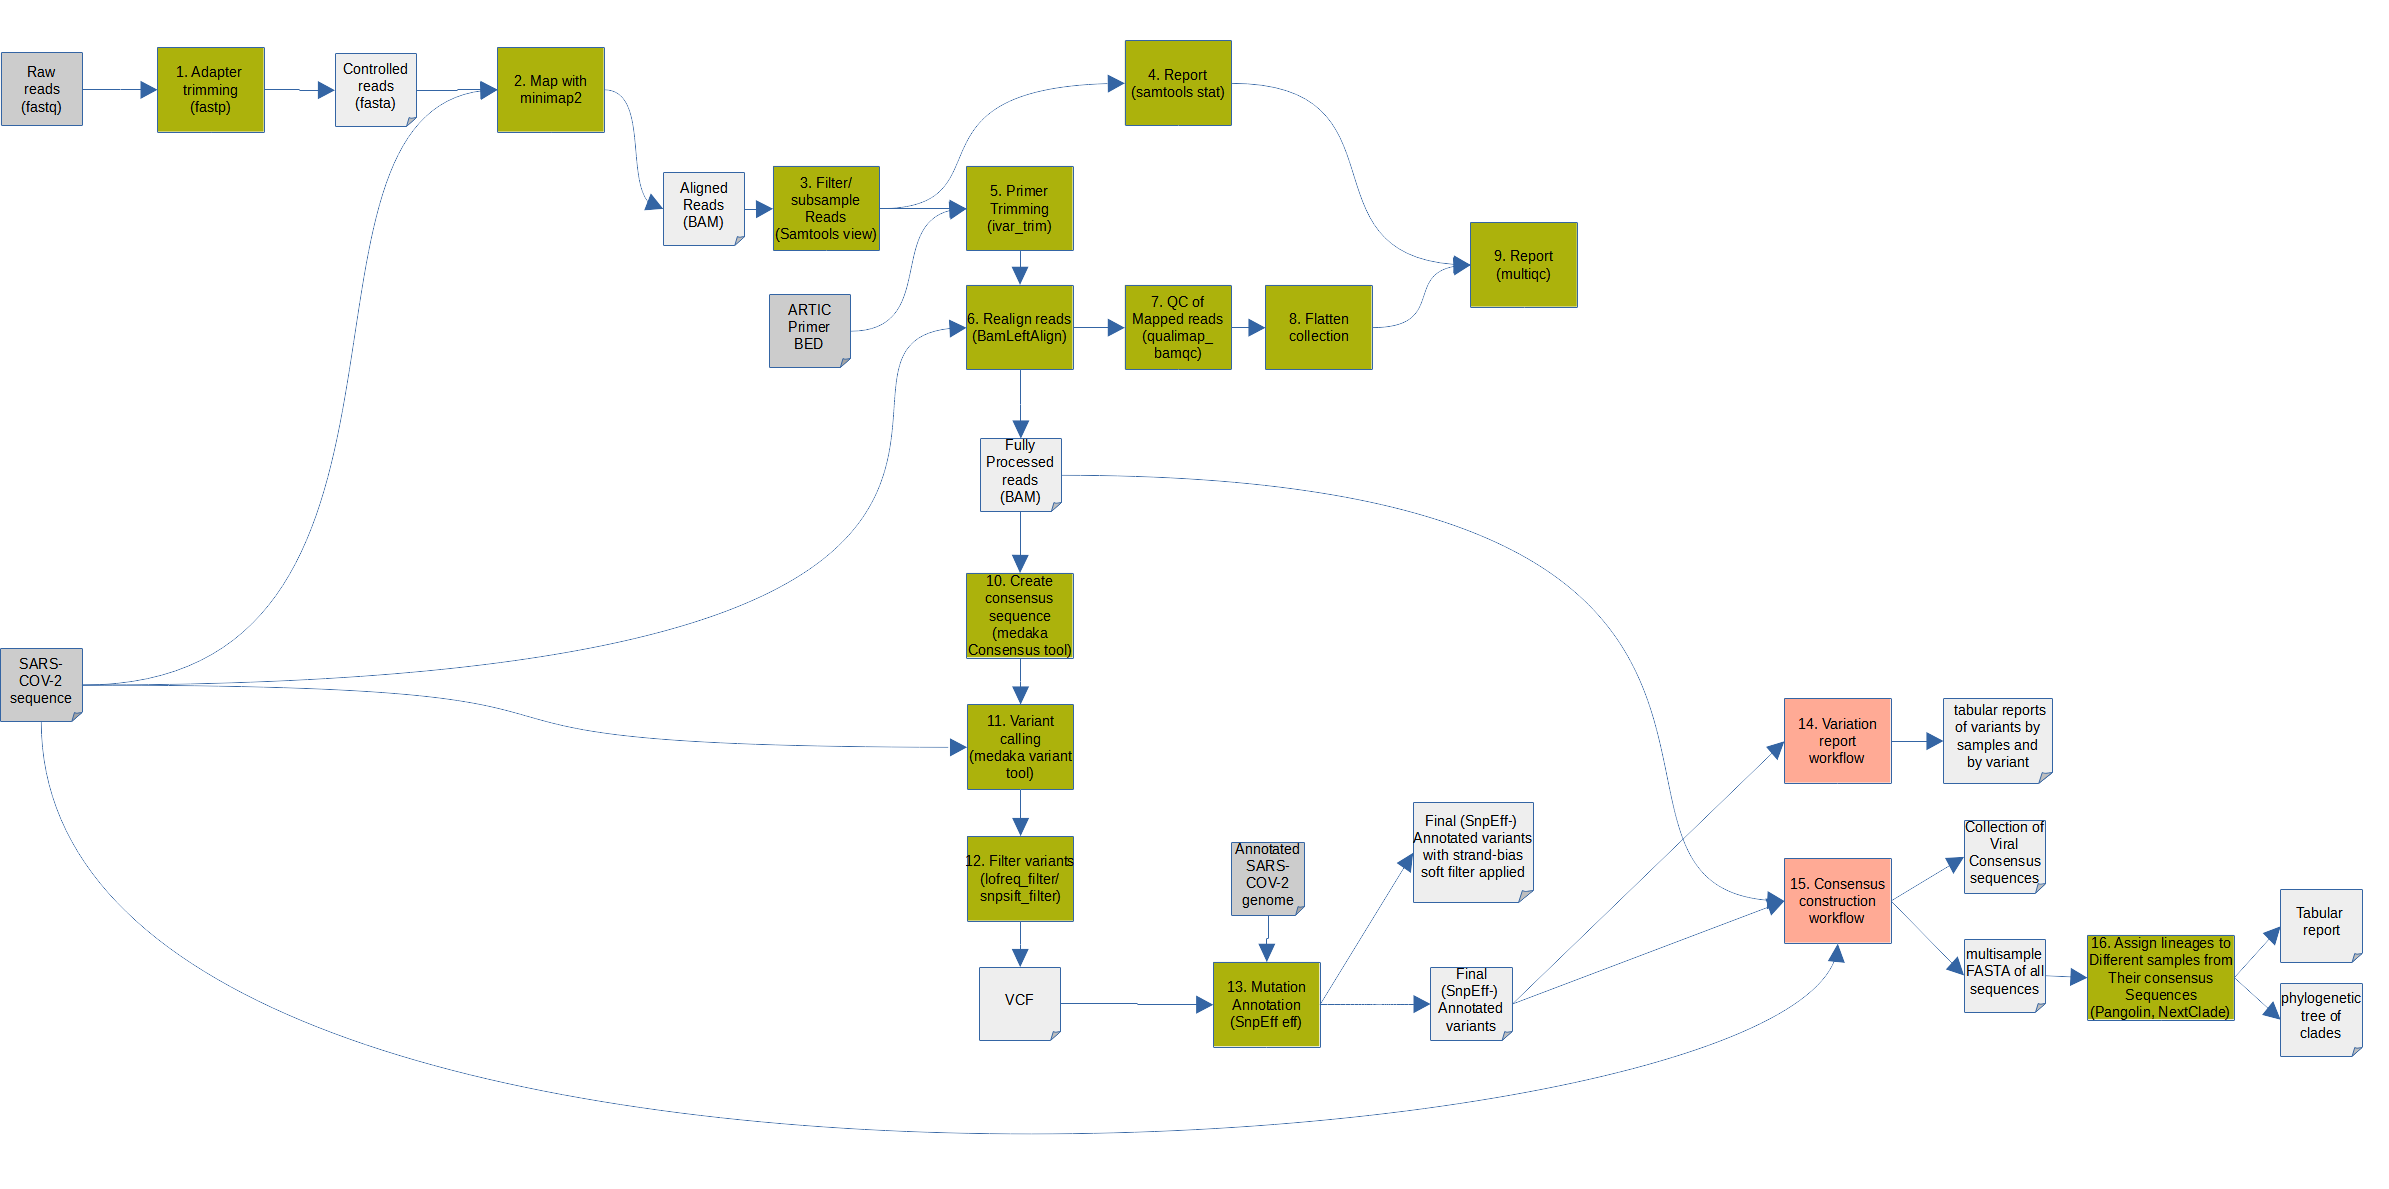
\includegraphics[width=1.4\textwidth]{figures/further/further-ont-wf.png}
            \captionof{figure}{One of four existing Galaxy workflow for SARS-CoV-2 clinical data surveillance for single-end reads data extracted with amplicon-based technique and sequenced with Nanopore sequencing approach.}
            \label{fig:further:ont-wf}
        \end{figure}
        \begin{figure}[ht!]
        	\centering
            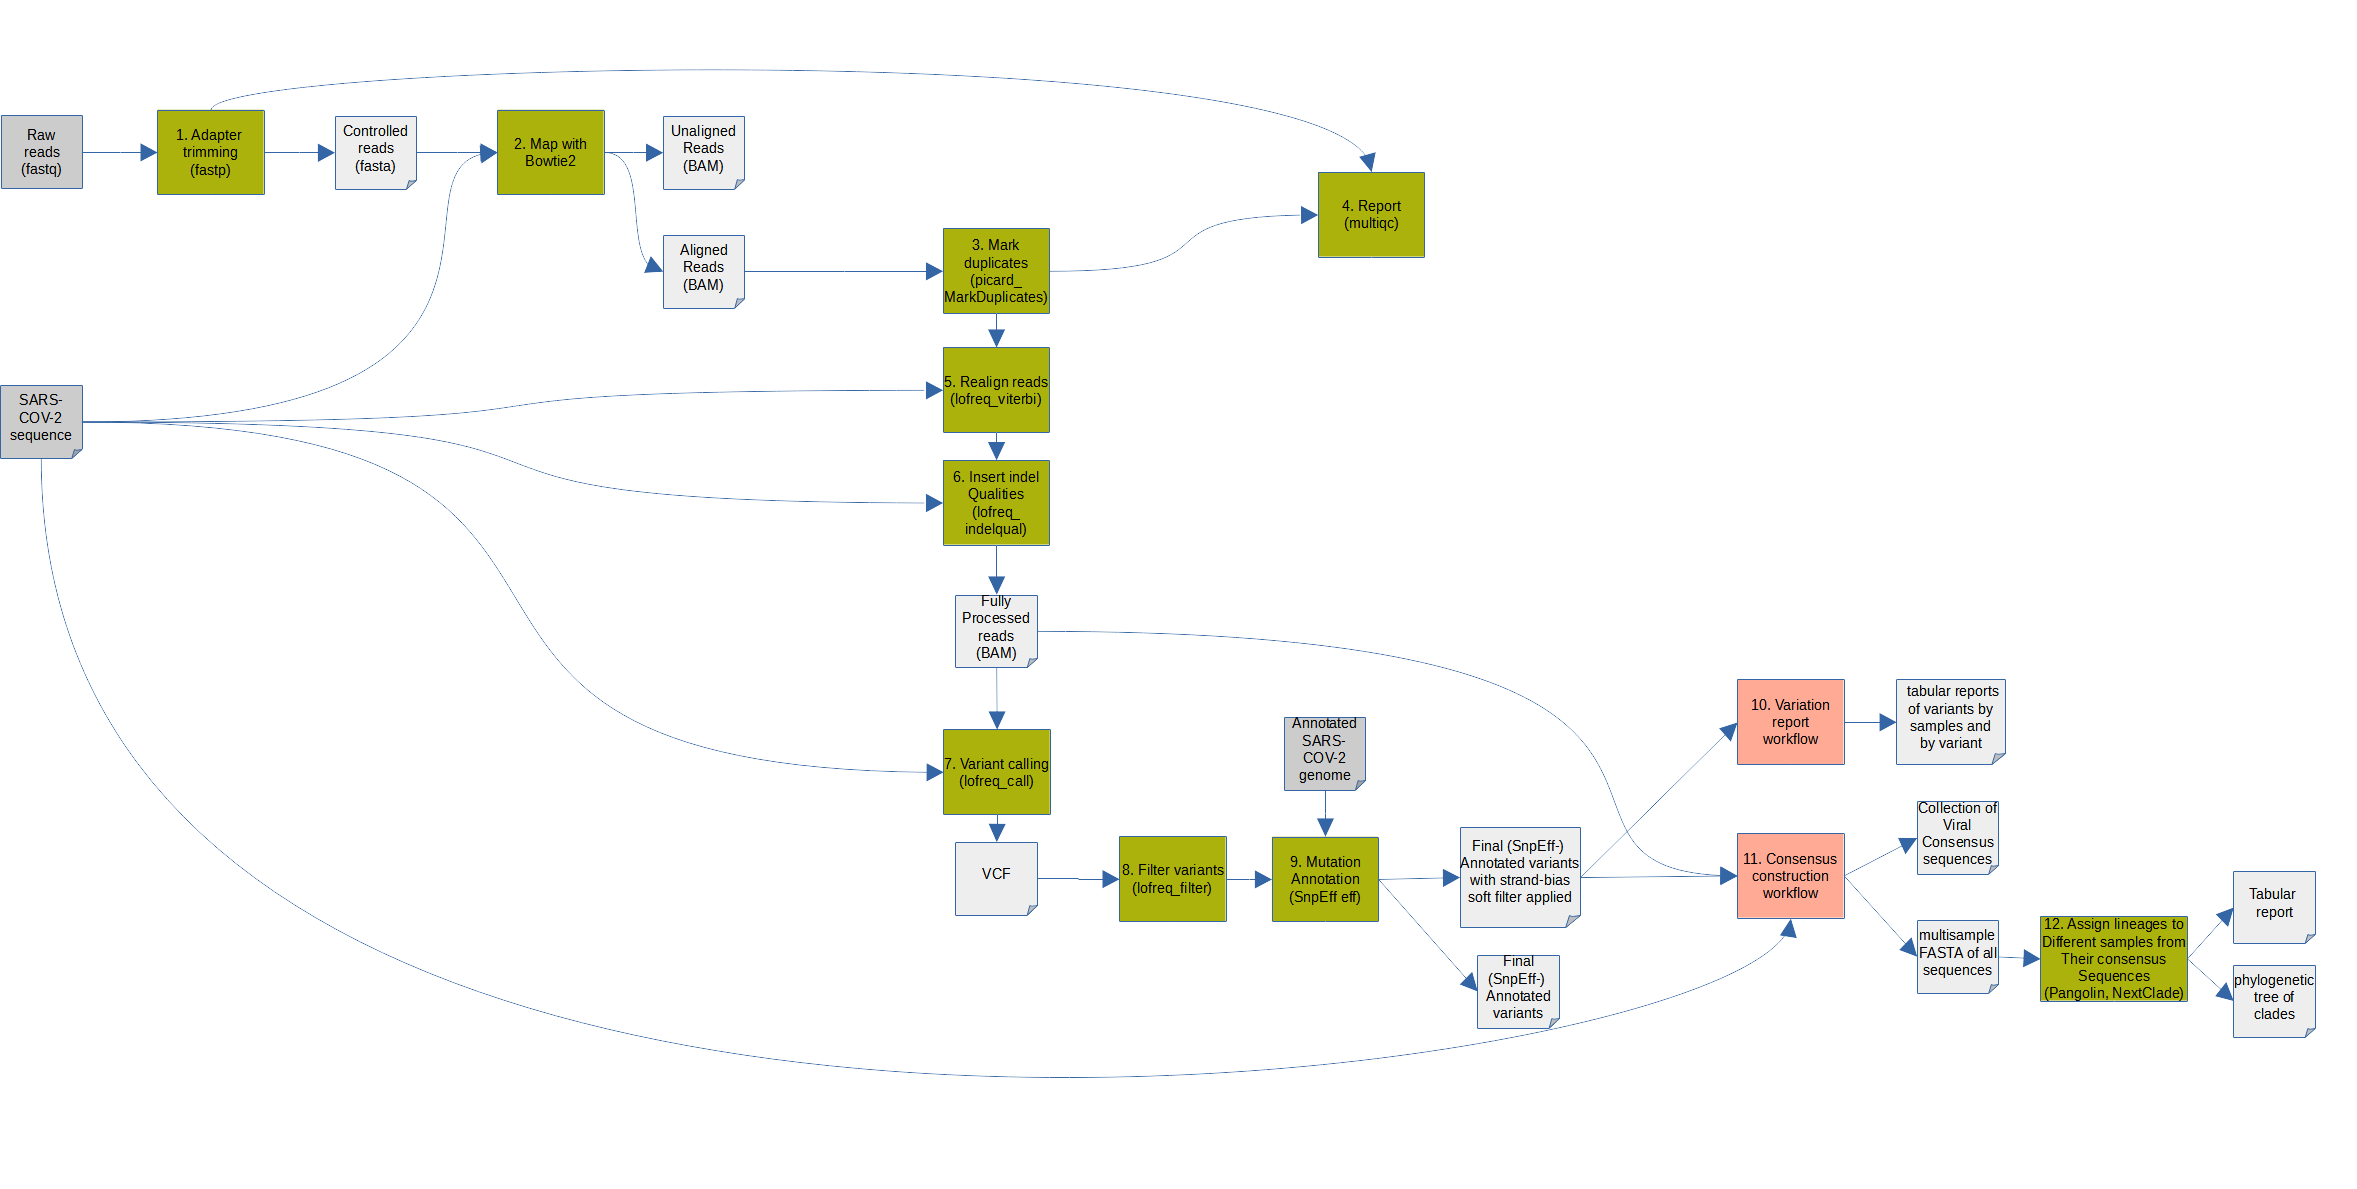
\includegraphics[width=1.4\textwidth]{figures/further/further-illumina-wf.png}
            \captionof{figure}{One of four existing Galaxy workflow for SARS-CoV-2 clinical data surveillance for single-end reads data extracted with metatranscriptomic-based technique and sequenced with Illumina sequencing approach.}
            \label{fig:further:illumina-wf}
        \end{figure}
        \vfill
        \end{landscape}
        
        
\clearpage

